\documentclass[tikz, border=0pt]{standalone}
\usepackage{tikz}

\begin{document}
	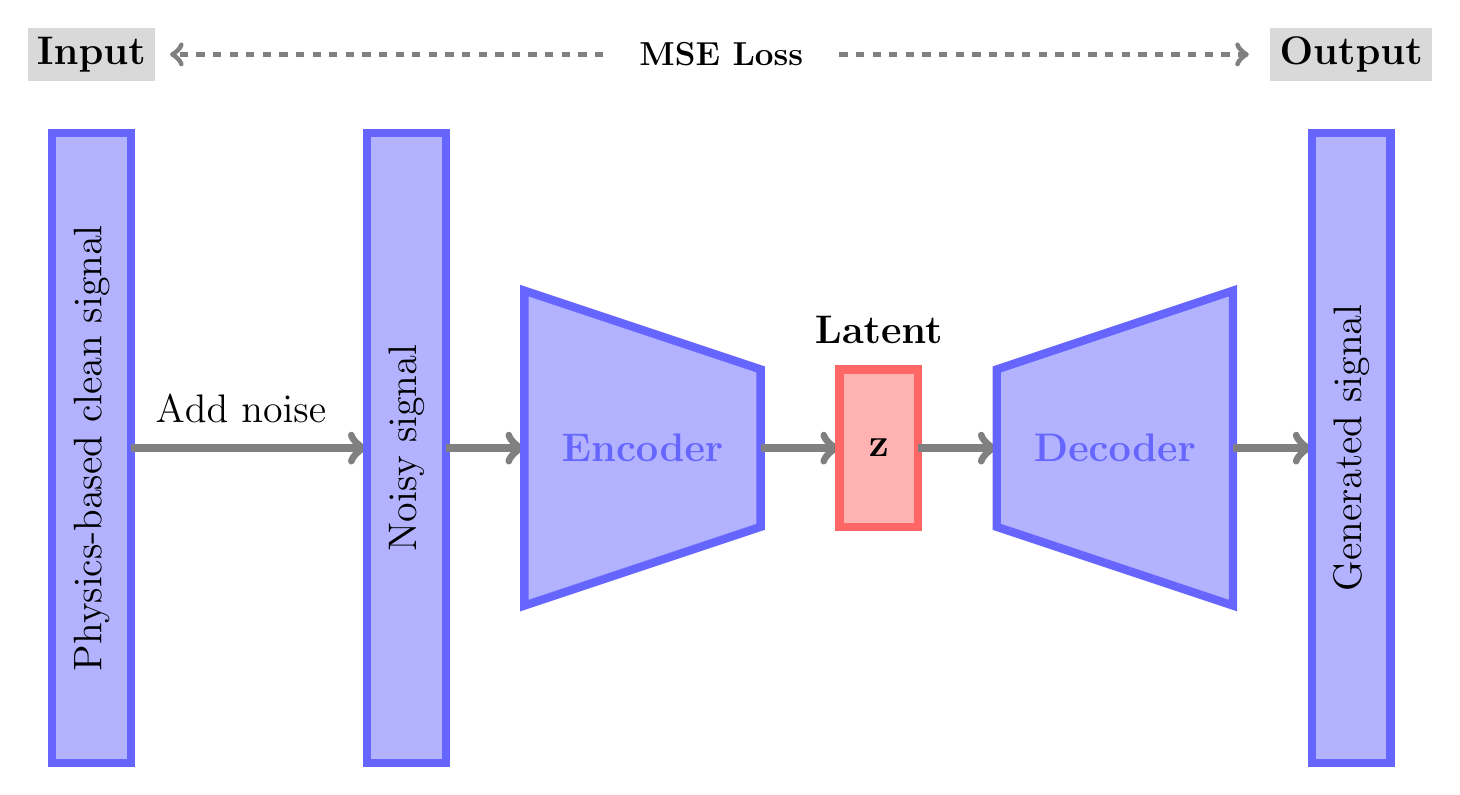
\begin{tikzpicture}
		\draw[fill=blue!30, draw=blue!60, line width=3pt] (0, 0) rectangle (1, 8);
		\node[font=\Large, rotate=90] at (0.5,4) {Physics-based clean signal};
		
		\node[font=\Large] at (2.4, 4.5) {Add noise};
		\draw[->, gray, thick, line width=3pt] (1, 4) -- (4, 4);
		
		\draw[fill=blue!30, draw=blue!60, line width=3pt] (4, 0) rectangle (5, 8);
		\node[font=\Large, rotate=90] at (4.5,4) {Noisy signal};
		
		\draw[->, gray, thick, line width=3pt] (5, 4) -- (6, 4);
		\draw[fill=blue!30, draw=blue!60, line width=3pt] (6,6) -- (6,2) -- (9,3) -- (9,5) -- cycle;
		\node[text=blue!60, font=\Large] at (7.5,4) {\textbf{Encoder}};
		
		\draw[->, gray, thick, line width=3pt] (9,4) -- (10,4);

		\draw[fill=red!30, draw=red!60, line width=3pt] (10, 3) rectangle (11, 5);
		\node[font=\Large] at (10.5, 4) {$\mathbf{z}$};
		\node[font=\Large] at (10.5, 5.5) {\textbf{Latent}};

		\draw[->, gray, thick, line width=3pt] (11, 4) -- (12, 4);

		\draw[fill=blue!30, draw=blue!60, line width=3pt] (12,3) -- (12,5) -- (15,6) -- (15,2) -- cycle;
		\node[text=blue!60, font=\Large] at (13.5,4) {\textbf{Decoder}};

		\draw[->, gray, thick, line width=3pt] (15, 4) -- (16, 4);

		\draw[fill=blue!30, draw=blue!60, line width=3pt] (16, 0) rectangle (17, 8);
		\node[font=\Large, rotate=90] at (16.5,4) {Generated signal};

		\node[text=black, font=\Large, fill=gray!30] at (0.5,9) {\textbf{Input}};
		\node[text=black, font=\Large, fill=gray!30] at (16.5,9) {\textbf{Output}};

		\draw[->, gray, thick, dashed, line width=2pt] (7, 9) -- (1.5, 9);
		\draw[->, gray, thick, dashed, line width=2pt] (10, 9) -- (15.2, 9);

		\node[text=black, font=\large] at (8.5,9) {\textbf{MSE Loss}};
	\end{tikzpicture}
\end{document}
